\documentclass[conference]{IEEEtran}
\IEEEoverridecommandlockouts

\usepackage{cite}
\usepackage{amsmath,amssymb,amsfonts}
\usepackage{amsbsy}
\usepackage{mathtools}
\usepackage{subfigure}
\usepackage{algorithmic}
\usepackage{graphicx}
\usepackage{textcomp}
\usepackage{xcolor}
\usepackage{tcolorbox}
\usepackage{textcomp}
\usepackage{float}
\usepackage{array}
\usepackage{siunitx}
\usepackage{tabularx}
\usepackage{listings}
\usepackage{accents}
\usepackage{nicematrix,tikz}
\usepackage{setspace}
\usepackage{colortbl} % For background colors in tables and matrices
\usepackage[colorlinks=false]{hyperref}
\def\BibTeX{{\rm B\kern-.05em{\sc i\kern-.025em b}\kern-.08em
    T\kern-.1667em\lower.7ex\hbox{E}\kern-.125emX}}

\setlength{\parindent}{0pt}

% Define the custom column type Y
\newcolumntype{Y}{>{\centering\arraybackslash} m{0.9cm}}

\definecolor{codeblue}{rgb}{0.2,0.2,0.6}
\definecolor{codegreen}{rgb}{0.133,0.545,0.133}
\definecolor{codegray}{rgb}{0.5,0.5,0.5}
\definecolor{codepurple}{rgb}{0.58,0,0.82}
\definecolor{backcolour}{rgb}{0.95,0.95,0.92}

\lstdefinestyle{mystyle}{
    backgroundcolor=\color{backcolour},
    commentstyle=\color{codegreen},
    keywordstyle=\color{codeblue},
    numberstyle=\tiny\color{codegray},
    stringstyle=\color{codepurple},
    basicstyle=\ttfamily\scriptsize,
    breakatwhitespace=false,
    breaklines=true,
    captionpos=b,
    keepspaces=true,
    numbers=none,
    numbersep=5pt,
    showspaces=false,
    showstringspaces=false,
    showtabs=false,
    tabsize=2
}
\lstset{style=mystyle}


% --------------------- Terminal Style ---------------------
% Define light theme colors
\definecolor{mygray}{rgb}{0.95, 0.95, 0.95}
\definecolor{myblue}{rgb}{0.65, 0.75, 0.85}
\definecolor{myblack}{rgb}{0, 0, 0}
\definecolor{myred}{rgb}{0.886, 0.529, 0.262}

% Define dark theme colors
\definecolor{mydarkgray}{rgb}{0.15, 0.15, 0.15}
\definecolor{myteal}{rgb}{0.1, 0.7, 0.7}
\definecolor{mywhite}{rgb}{1, 1, 1}

% Choose the theme here
\colorlet{backgroundcolor}{mygray}
\colorlet{bordercolor}{myblue}
\colorlet{textcolor}{myblack}
\colorlet{numbercolor}{myred}

% Customize listings style without background or frame
\lstset{
    basicstyle=\ttfamily\footnotesize\color{textcolor}, % Font style and size
    keywordstyle=\color{orange}\bfseries,              % Style for keywords
    commentstyle=\color{green}\itshape,                % Style for comments
    stringstyle=\color{purple},                        % Style for strings
    identifierstyle=\color{textcolor},                 % Style for identifiers
    numberstyle=\tiny\color{numbercolor},                % Style for line numbers
    columns=fullflexible,                              % Flexible column width
    breaklines=true,                                   % Automatic line breaking
    breakatwhitespace=true,                            % Only break lines at white spaces
    postbreak=\mbox{\textcolor{red}{$\hookrightarrow$}\space}, % Break symbol
    showstringspaces=false,                            % Do not show spaces in strings
    numbers=left,                                      % Line numbers on the left
    stepnumber=1,                                      % Step number for line numbers
    numbersep=4pt,                                    % Separation between numbers and code
    frame=none,                                        % No frame, handled by tcolorbox
    xleftmargin=5pt,                                  % Space for line numbers
}

% Define tcolorbox with rounded corners
\newtcolorbox{mylistingbox}[1][]{colback=backgroundcolor, colframe=bordercolor, arc=3mm,
                                  boxrule=0.4mm, left=10pt, right=4pt, top=2pt,
                                  bottom=2pt, boxsep=0pt, #1}

% ----------------------------------------------------------

% Define a custom color for the background
\definecolor{lightblue}{rgb}{0.8,0.85,1.0}

\title{Robotics and Mechatronics\\
{\LARGE Homework Six}
}

\author{\IEEEauthorblockN{Mohammad Montazeri}
    \IEEEauthorblockA{\textit{School of Mechanical Engineering} \\
        \textit{College of Engineering, University of Tehran}\\
        Tehran, Iran; 810699269 \\
        mohammadmontazeri@ut.ac.ir}
}

\begin{document}
\maketitle

\begin{abstract}
    This report explores the use of machine learning  and neural networks in robotics, focusing on backpropagation, perceptron learning, CNNs, MLPs for solving IKP, and SVMs. These techniques improve robotic precision and autonomy by enhancing data processing and decision-making. They also facilitate the robotic issues unsolvable by classic analytical approaches.
\end{abstract}

\begin{IEEEkeywords}
    Neural Network, model, learning, training, loss, backpropagation, prediction, error
\end{IEEEkeywords}

\section{Introduction}
Machine learning has become essential in robotics for improving control and decision-making systems. Backpropagation is a key algorithm for training neural networks by minimizing prediction errors. Perceptron learning serves as the foundation for creating simple binary classifiers.

Convolutional Neural Networks (CNNs) are crucial for visual perception tasks, enabling robots to process and recognize spatial data. The Inverse Kinematics Problem (IKP), which determines joint angles for desired robot positions, can be effectively solved using Multi-Layer Perceptrons (MLPs).

Support Vector Machines (SVMs) offer robust solutions for classifying data by identifying the optimal separating hyperplane. This report provides an overview of these techniques and their applications in robotics, highlighting their role in enhancing robotic functionality and autonomy.
\vspace{8px}

\section{Problem 1: Back Propagation}
In neural network notations, we can present the $z_i^{(j)}$ and $a_i^{(j)}$ respectively as the input and output of the $i$-th neuron on the $j$-th layer. If we present the predicted outcomes of each neuron on the the output layer of the network as $\hat{O}_i$ for $i=1, 2$ and the true expected outcome as $O_i$, we can write the forward path for the network and calculate total error as below.
\begin{figure}[htbp]
    \centerline{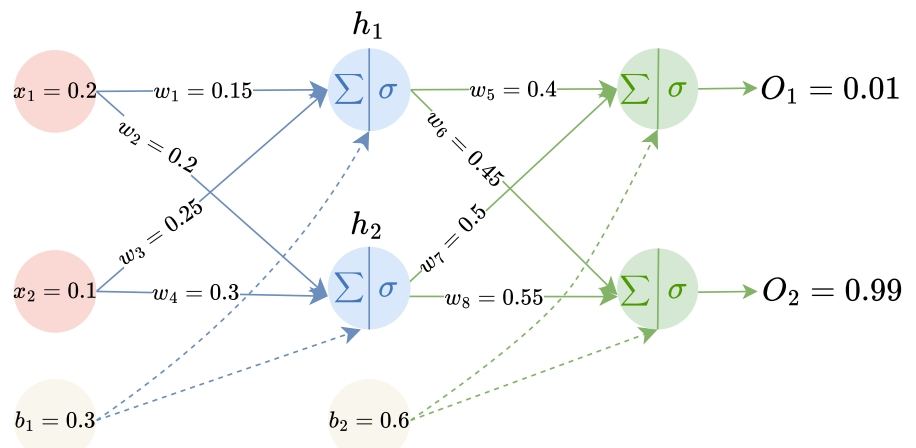
\includegraphics[width=0.45\textwidth]{figures/prob1.jpeg}}
    \caption{Architecture of the neural network with its initial values.}
    \label{fig:prob1}
\end{figure}
\vspace{4px}

\subsection*{a) Forward Path (feedforward)}
Calculate the input to each hidden node or output node and apply an activation function (e.g., sigmoid) to each sum.
\begin{align*}
     & z_1^{(1)} = w_1 x_1 + w_3 x_2 + b_1 = 0.15 \times 0.2 + 0.25 \times 0.1 + 0.3              \\
     & a_1^{(1)} = \sigma(z_1^{(1)}) = \sigma(0.355) = \dfrac{1}{1+\mathrm{e}^{-0.355}} = 0.58782 \\
     & z_2^{(1)} = w_2 x_1 + w_4 x_2 + b_1 = 0.2 \times 0.2 + 0.3 \times 0.1 + 0.3                \\
     & a_2^{(1)} = \sigma(z_2^{(1)}) = \sigma(0.37) = \dfrac{1}{1+\mathrm{e}^{-0.37}} = 0.59145
\end{align*}
\hrule
\begin{small}
    \begin{align*}
         & z_1^{(2)} = w_5 a_1^{(1)} + w_7 a_2^{(1)} + b_2 = 0.4 \times 0.5878 + 0.5 \times 0.5914 + 0.6   \\
         & a_1^{(2)} = \sigma(z_1^{(2)}) = \sigma(1.13082) = \dfrac{1}{1+\mathrm{e}^{-1.13082}} = 0.75599  \\
         & z_2^{(2)} = w_6 a_1^{(1)} + w_8 a_2^{(1)} + b_2 = 0.45 \times 0.5878 + 0.55 \times 0.5914 + 0.6 \\
         & a_2^{(2)} = \sigma(z_2^{(2)}) = \sigma(1.18978) = \dfrac{1}{1+\mathrm{e}^{-1.18978}} = 0.76670
    \end{align*}
\end{small}
\begin{align}
     & \rightarrow \hat{O}_1 = a_1^{(2)} = 0.75599 \\
     & \rightarrow \hat{O}_2 = a_2^{(2)} = 0.76670
\end{align}

Given the target values \(
O_1 = 0.01
\) and \(
O_2 = 0.99
\), we can calculate squared errors and sum them.
\begin{align*}
    E_1 & = |O_1 - \hat{O}_1| = |0.75599 - 0.01| = 0.74599 \nonumber \\
    E_2 & = |O_2 - \hat{O}_2| = |0.76670 - 0.99| = 0.2233 \nonumber  \\
\end{align*}

Assuming the cost function specified for this problem to be \textit{sum of squared errors} (SSE), we can find the total loss like\footnote{It should be noted that some resources \cite{b6} have a gain of $0.5$ in SSE loss formula which helps simplify the equation when a coefficient of 2 is multiplied in it while differentiating in backpropagation process. Although not accordant with some other references \cite{b7}, this notation is selected in this problem.}:
\begin{gather}
    J(w, b) = \frac{1}{2} \sum_{q=1}^{2} \left\| h_{w, b}^q(x) - y^q \right\|^2 \rightarrow \mathcal{L}_{SSE} = 0.5 \left(E_1^2 + E_2^2\right) \nonumber \\
    E_{tot} = 0.5 (0.55650 + 0.04986) = \mathbf{0.30318}
\end{gather}

\subsection*{b) Backward Path (back-propagation)}
The overall procedure for updating the weights in such a network is like:
\begin{itemize}
    \item Compute the error gradient with respect to the output layer: \[ \delta_1 = (\hat{O}_1 - O_1) \cdot \sigma^\prime(W_5 h_1 + W_7 h_2 + b_2) \] \[ \delta_2 = (\hat{O}_2 - O_2) \cdot \sigma^\prime(W_6 h_1 + W_8 h_2 + b_2) \] where $(\sigma^\prime)$ is the derivative of the activation function (e.g., sigmoid).
    \item Update the weights for the output layer: \[ W_5 \leftarrow W_5 - \text{learning rate} \cdot \delta_1 \cdot h_1 \] \[ W_6 \leftarrow W_6 - \text{learning rate} \cdot \delta_2 \cdot h_1 \] \[ W_7 \leftarrow W_7 - \text{learning rate} \cdot \delta_1 \cdot h_1 \] \[ W_8 \leftarrow W_8 - \text{learning rate} \cdot \delta_2 \cdot h_2 \]
    \item Compute the error gradient with respect to the hidden layer: \[ \delta_{h1} = (\delta_1 \cdot W_5 + \delta_2 \cdot W_6) \cdot \sigma^\prime(W_1x_1 + W_3x_2 + b_1) \] \[ \delta_{h2} = (\delta_1 \cdot W_7 + \delta_2 \cdot W_8) \cdot \sigma^\prime(W_2x_1 + W_4x_2 + b_1) \]
    \item Update the weights for the hidden layer: \[ W_1 \leftarrow W_1 - \text{learning rate} \cdot \delta_{h1} \cdot x_1 \] \[ W_2 \leftarrow W_2 - \text{learning rate} \cdot \delta_{h2} \cdot x_1 \] \[ W_3 \leftarrow W_3 - \text{learning rate} \cdot \delta_{h1} \cdot x_2 \] \[ W_4 \leftarrow W_4 - \text{learning rate} \cdot \delta_{h2} \cdot x_2 \]
\end{itemize}

In this problem, to update only $w_4$ and $w_5$, we need to differentiate the total loss with respect to them. For this matter, we take learning rate $\eta = 1$ and note that the derivative of the sigmoid function is as below \cite{b3}.
\begin{align}
    \sigma^\prime (z) = \sigma(z) \left(1 - \sigma(z)\right)
\end{align}

\subsubsection{Updating $W_5$}

{\setlength{\jot}{8pt}
    \begin{align}
        \frac{\partial \mathcal{L}}{\partial w_5} & = \frac{1}{2} \left[\frac{\partial E_1^2}{\partial w_5} + \frac{\partial E_2^2}{\partial w_5} \right]= E_1\frac{\partial E_1}{\partial w_5}                    \\
                                                  & = E_1 \,\, \frac{\partial E_1}{\partial a_1^{(2)}}    \quad   \frac{\partial a_1^{(2)}}{\partial z_1^{(2)}}    \quad   \frac{\partial z_1^{(2)}}{\partial w_5} \\
                                                  & = E_1 \times 1 \times a_1^{(2)} \left(1 - a_1^{(2)}\right)  \times a_1^{(1)}                                                                                   \\
                                                  & = 0.74599 \times 0.75599 (1 - 0.75599) \times 0.58782 \nonumber                                                                                                \\
                                                  & = \mathbf{0.08089115564}
    \end{align}}

\begin{align*}
    \left. w_5\right|_{new} = \left. w_5\right|_{old} - \eta \nabla_{w_5} \mathcal{L} = 0.4 - \frac{\partial \mathcal{L}}{\partial w_5} = \mathbf{0.31911}
\end{align*}

\subsubsection{Updating $W_4$}
\begin{align}
    \frac{\partial \mathcal{L}}{\partial w_4}  = & \, \frac{1}{2} \left[\frac{\partial E_1^2}{\partial w_4} + \frac{\partial E_2^2}{\partial w_4} \right]= \left[E_1\frac{\partial E_1}{\partial w_4} + E_2 \frac{\partial E_2}{\partial w_4}\right]                                                                                                                   \\
    =                                            & \left[E_1 \,\, \frac{\partial E_1}{\partial a_1^{(2)}}    \quad   \frac{\partial a_1^{(2)}}{\partial z_1^{(2)}}    \quad   \frac{\partial z_1^{(2)}}{\partial a_2^{(1)}}     \quad  \frac{\partial a_2^{(1)}}{\partial z_2^{(1)}}   \quad    \frac{\partial z_2^{(1)}}{\partial w_4}    \right. \nonumber           \\
                                                 & \left. \, + \, E_2 \,\, \frac{\partial E_2}{\partial a_2^{(2)}}   \quad    \frac{\partial a_2^{(2)}}{\partial z_2^{(2)}}  \quad     \frac{\partial z_2^{(2)}}{\partial a_2^{(1)}}    \quad   \frac{\partial a_2^{(1)}}{\partial z_2^{(1)}}     \quad  \frac{\partial z_2^{(1)}}{\partial w_4}     \right] \nonumber
\end{align}

\begin{small}
    \begin{align*}
        \frac{\partial \mathcal{L}}{\partial w_4}  = & \left[E_1 \times 1 \times a_1^{(2)} \left(1 - a_1^{(2)}\right)  \times w_7 \times a_2^{(1)} \left(1 - a_2^{(1)}\right) \times x_2 \right.   \\
                                                     & \left. + E_2 \times 1 \times a_2^{(2)} \left(1 - a_2^{(2)}\right) \times w_8 \times a_2^{(1)} \left(1 - a_2^{(1)}\right) \times x_2 \right]
    \end{align*}
\end{small}

\begin{align*}
    \frac{\partial \mathcal{L}}{\partial w_4}  = & \, 0.74599 \times 0.75599 (1 - 0.75599) \times 0.5 \\
                                                 & \times 0.59145 (1 - 0.59145) \times 0.1 +          \\
                                                 & \, 0.2233 \times 0.76670 (1 - 0.76670) \times 0.55 \\
                                                 & \times 0.59145 (1 - 0.59145) \times 0.1            \\
    =                                            & \, \mathbf{0.00219343754}
\end{align*}

\begin{align*}
    \left. w_4\right|_{new} = \left. w_4\right|_{old} - \eta \nabla_{w_4} \mathcal{L} = 0.3 - \frac{\partial \mathcal{L}}{\partial w_4} = \mathbf{0.29781}
\end{align*}
\vspace{21px}

\section{Problem 2: Perceptron Learning}
\begin{figure}[htbp]
    \centerline{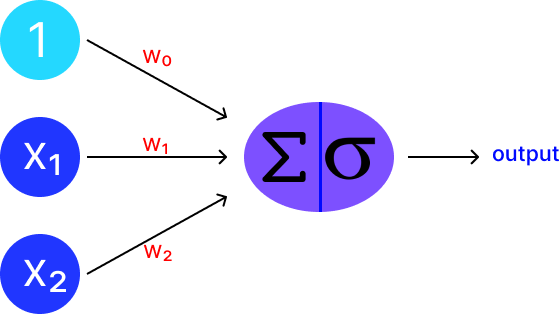
\includegraphics[width=0.44\textwidth]{figures/perceptron.png}}
    \caption{Architecture of the perceptron used in problem 2.}
    \label{fig:prob2}
\end{figure}
\subsection*{a) Creating perceptron manually}
With the given training samples, our intuition is bent towards the fact that the perceptron outputs positively for inputs which together are greater than or equal to 3. This satisfies all 3 examples. So, the simplest way to put this in perceptron is by giving the values below to the weights and bias.

\begin{align}
     & w_0 = -3 \hspace{20px}                 & w_1 = w_2 = 1 \nonumber   \\
     & z = \sum_{0}^{2} w_i x_i \hspace{20px} & \sigma(z) = \begin{cases}
                                                                +1, & z \ge 0 \\
                                                                -1, & z < 0
                                                            \end{cases}
\end{align}

\subsection*{b) Implementing learning algorithm}
Now assuming we are unaware of the true weights of this perceptron and unable to derive them by mind, we use the following algorithm to modify weights step by step.
\begin{itemize}
    \item Let \begin{footnotesize}
              $$
                  \mathcal{D}=\left(\left\langle\mathbf{x}^{[1]}, y^{[1]}\right\rangle, \ldots,\left\langle\mathbf{x}^{[n]}, y^{[n]}\right\rangle\right) \in\left(\mathbb{R}^m \times\{0,1\}\right)^n
              $$
          \end{footnotesize}
    \item Initialize $\mathbf{w}=[w_0, w_1, w_2]:=[-1, 1, 0.5]$
    \item For every training epoch: \begin{itemize}
              \item For every $\left\langle\mathbf{x}^{[i]}, y^{[i]}\right\rangle \in \mathcal{D}$ : \begin{enumerate}
                        \item $\hat{y}^{[i]}:=\sigma\left(\mathbf{x}^{[i] \top} \mathbf{w}\right)$
                        \item err $:=\left(y^{[i]}-\hat{y}^{[i]}\right)$
                        \item $\mathbf{w}:=\mathbf{w}+\operatorname{err} \cdot \mathbf{x}^{[i]}$
                    \end{enumerate}
          \end{itemize}
\end{itemize}

To implement this, \textit{\underline{Python}} is used to automate the learning procedure. The code provided for this matter is appended to this report while its result shows:

% Use tcolorbox for the round corners and custom border
\begin{mylistingbox}
    \begin{lstlisting}[language=Python]
    --- epoch 1 ---
    w0, w1, w2 = [-1, 1, 0.5]
    w0, w1, w2 = [-1, 1, 0.5]
    w0, w1, w2 = [-1.5, 1.0, -0.5]
    w0, w1, w2 = [-1.5, 1.0, -0.5]
    total error = 2
    --- epoch 2 ---
    w0, w1, w2 = [-1.5, 1.0, -0.5]
    w0, w1, w2 = [-2.0, 0.5, 0.0]
    w0, w1, w2 = [-2.0, 0.5, 0.0]
    w0, w1, w2 = [-1.5, 1.5, 0.5]
    total error = 4
    --- epoch 3 ---
    w0, w1, w2 = [-1.5, 1.5, 0.5]
    w0, w1, w2 = [-1.5, 1.5, 0.5]
    w0, w1, w2 = [-1.5, 1.5, 0.5]
    w0, w1, w2 = [-1.5, 1.5, 0.5]
    total error = 0
\end{lstlisting}
\end{mylistingbox}

This shows that with the initial weights of \texttt{w0, w1, w2 = [-1, 1, 0.5]} and a learning rate of \texttt{0.5}, perceptron reaches an admirable answer for weights, in just 3 epochs. Dividing the learning rate by 2 causes the perceptron to reach another true answer with one epoch less, like:
\begin{mylistingbox}
    \begin{lstlisting}[language=Python]
    --- epoch 1 ---
    w0, w1, w2 = [-1, 1, 0.5]
    w0, w1, w2 = [-1, 1, 0.5]
    w0, w1, w2 = [-1.25, 1.0, 0.0]
    w0, w1, w2 = [-1.25, 1.0, 0.0]
    total error = 2
    --- epoch 2 ---
    w0, w1, w2 = [-1.25, 1.0, 0.0]
    w0, w1, w2 = [-1.25, 1.0, 0.0]
    w0, w1, w2 = [-1.25, 1.0, 0.0]
    w0, w1, w2 = [-1.25, 1.0, 0.0]
    total error = 0
    \end{lstlisting}
\end{mylistingbox}

These results \_although true\_ were obtained using a learning algorithm which updates weights like below and was derived from \cite{b6}.
\begin{align}
    \mathbf{w}:=\mathbf{w}+\operatorname{y_{true}} \cdot \mathbf{x}^{[i]}
\end{align}

After changing the code a little bit to use our own previously-discussed updating rule derived from \cite{b7} as $\mathbf{w}:=\mathbf{w}+\operatorname{err} \cdot \mathbf{x}^{[i]}$, we get the following result which leads to final weights of \\
\begin{large}
    \texttt{\textbf{w0, w1, w2 = [-2, 2, 0.5]}}
\end{large}
\begin{mylistingbox}
    \begin{lstlisting}[language=Python]
    --- epoch 1 ---
    w0, w1, w2 = [-1.0, 3.0, -0.5]
    total error = 4
    --- epoch 2 ---
    w0, w1, w2 = [-2.0, 2.0, 0.5]
    total error = 2
    --- epoch 3 ---
    w0, w1, w2 = [-2.0, 2.0, 0.5]
    total error = 0
\end{lstlisting}
\end{mylistingbox}
\vspace{15px}

\section{Problem 3: SVM}
Support Vector Machines are powerful supervised learning algorithms for both classification and regression. It is a discriminative classifier that is formally defined by a separating hyperplane. So given labelled training data, the algorithm outputs an optimal hyperplane that categorizes new examples.

\subsection*{a) Linear Separability}
In this 1D space, it's impossible to draw a single line that separates the positive and negative samples. Therefore, the data is not linearly separable. SVM proposes a solution called \textit{Kernel Trick} which helps moving the data into a higher dimensional space where the data samples would be separated with a hyper-plane.

\subsection*{b) Kernel and Transfer Functions}
Given the kernel function:
\[
    K(x_1, x_2) = \cos\left(\frac{\pi}{4}x_1\right)\cos\left(\frac{\pi}{4}x_2\right) + \sin\left(\frac{\pi}{4}x_1\right)\sin\left(\frac{\pi}{4}x_2\right)
\]

This looks like the expression of the cosine of the difference of two angles, which suggests a trigonometric transformation. We can use this to find the transformation function \( \phi \).

Rewriting the kernel function using the trigonometric identity for the cosine of a difference gives
\[
    \cos(A - B) = \cos(A)\cos(B) + \sin(A)\sin(B)
\]

Let \( A = \frac{\pi}{4}x_1 \) and \( B = \frac{\pi}{4}x_2 \). Thus,
\[
    K(x_1, x_2) = \cos\left(\frac{\pi}{4}x_1 - \frac{\pi}{4}x_2\right) = \cos\left(\frac{\pi}{4}(x_1 - x_2)\right)
\]

Knowing
\begin{align}
    K(\mathbf{x_1}, \mathbf{x_2}) = \mathbf{\phi(x_1)} \cdot \mathbf{\phi(x_2)}
\end{align}


we can deduce that the transformation function \( \phi \) that maps 1D points to a 2D space is given by:
\begin{align}
    \boldsymbol{\phi}(x) = \left[ \cos\left(\frac{\pi}{4}x\right), \sin\left(\frac{\pi}{4}x\right) \right]
\end{align}


\subsection*{c) Points and Support Vectors Displayed}
Using a Python script which is appended to this file, we can transfer the data points from the 1-D to 2-D space and plot it. We can also use \texttt{svm} API from \texttt{sklearn} package to fit SVM to these points and plot the separation line along with its gutters (support vectors). As Figure~\ref{fig:prob3} shows the result, it can be seen that some data points happen to overlap on each other wen transferred to 2D space; thus, each point has a number label which shows how many points actually exist on that coordinate. With this module, in addition to all above, we can derive the equation for the separating line as: \\
\texttt{The equation of the separator line is: \\ y = 0.00x + -0.00}

\begin{figure}[htbp]
    \centerline{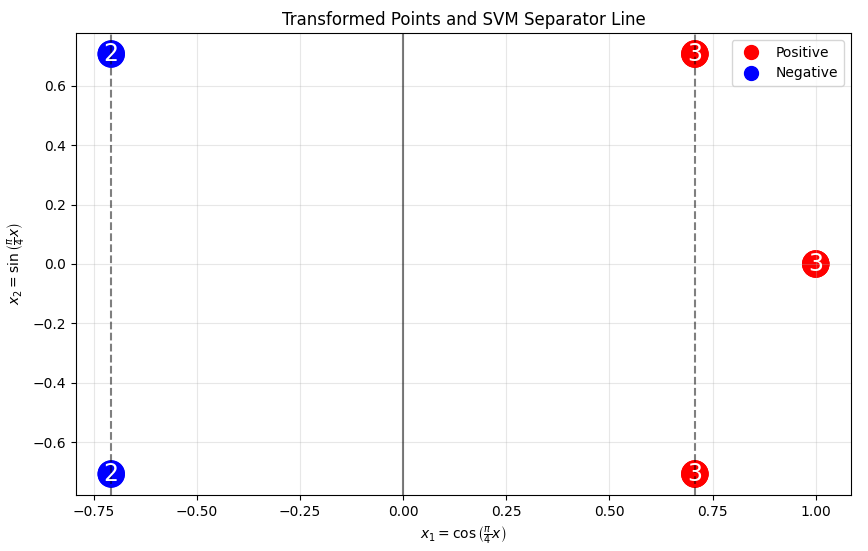
\includegraphics[width=0.465\textwidth]{figures/prob3.png}}
    \caption{Transformed points in 2D space with separation and supporting lines.}
    \label{fig:prob3}
\end{figure}

\subsection*{d) Equation of the Separator Line}
Figure~\ref{fig:prob3} shows that the nearest samples of two classes are kind of symmetrically spread about the vertical line $y = 0$ which happens to be the line that causes the biggest margin between the two classes. Therefore, as derived in the previous section, the separator line in the transformed space is obtained as a linear function like:
\begin{align}
    \Large
    \mathbf{X_1 = 0}
\end{align}
\vspace{12px}

\section{Problem 4: CNN Forward Process}
The inputs, filter weights and other parameters of the convolutional neural network in this problem are specified to me as shown in Figure~\ref{fig:prob4}.
\begin{figure}[htbp]
    \centerline{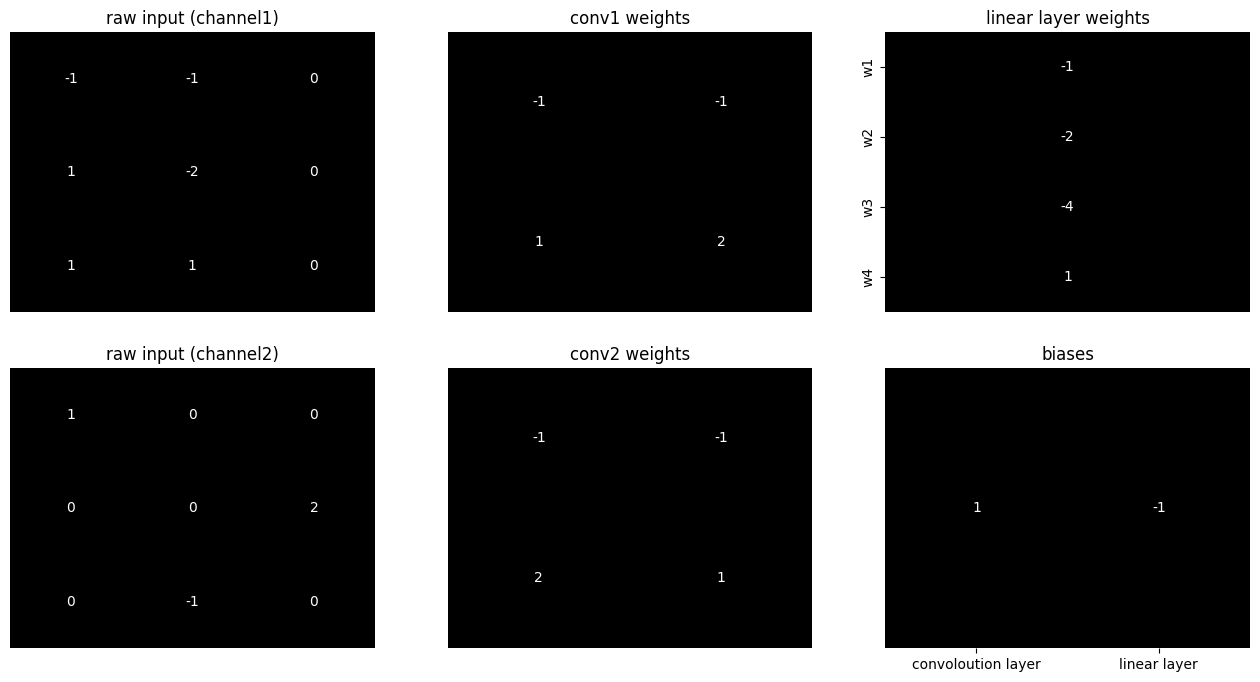
\includegraphics[width=0.45\textwidth]{figures/prob4.png}}
    \caption{The specified parameters to the author's specific CNN.}
    \label{fig:prob4}
\end{figure}

In other words, after adding one row/column of zero padding around (all over the) inputs, we'll have the following channels as the $2@(5\times5)$ input image.
\begin{align}
    \begin{bmatrix}
        0 & 0  & 0  & 0 & 0 \\
        0 & -1 & -1 & 0 & 0 \\
        0 & 1  & -2 & 0 & 0 \\
        0 & 1  & 1  & 0 & 0 \\
        0 & 0  & 0  & 0 & 0
    \end{bmatrix} \hspace{20px} \begin{bmatrix}
                                    0 & 0 & 0  & 0 & 0 \\
                                    0 & 1 & 0  & 0 & 0 \\
                                    0 & 0 & 0  & 2 & 0 \\
                                    0 & 0 & -1 & 0 & 0 \\
                                    0 & 0 & 0  & 0 & 0
                                \end{bmatrix}
\end{align}

At first we need to convolve this input channels with the filters \underline{below}, a bias of \underline{1} and a stride of \underline{1} for each. Then we need to add them together to get a uni-channel output.
\begin{align}
    \begin{bmatrix}
        -1 & -1 \\
        1  & 2
    \end{bmatrix} \hspace{20px} \begin{bmatrix}
                                    -1 & -1 \\
                                    2  & 1
                                \end{bmatrix}
\end{align}

To do so, we use the following convolution rule. (Note that this equation is used for each convolution \_with a filter and its corresponding input channel together\_ separately.)
\begin{equation}
    z = \mathbf{x} \cdot \mathbf{w} + b
\end{equation}
where $z$ is the scalar output of one filtered part, $\mathbf{x}$ is the $2\times2$ section of the input, $\mathbf{w}$ is the $2\times2$ filter weight matrix, and $b$ is the bias.

Therefore, we can calculate the first or the top-left $(0, 0)$ index of the convolved result like:
\begin{align*}
    z_{(0, 0)} = & \, (0\times-1 + 0\times-1 + 0\times1 + -1\times2 + 1)   \\
                 & + (0\times-1 + 0\times-1 + 0\times2 + 1\times1 + 1) = 1
\end{align*}
With the same procedure, we obtain
\begin{align}
    \begin{bmatrix}
        1 & 1 & 1 & 2 \\
        4 & 0 & 3 & 6 \\
        3 & 5 & 1 & 0 \\
        1 & 1 & 2 & 2
    \end{bmatrix}
\end{align}

Dividing the $4\times4$ result into 4 of $2\times2$ pieces and extracting each one's maximum value, we can achieve:
{\renewcommand{\arraystretch}{1.4} % Increase vertical padding
\newcolumntype{L}{>{\hspace{4pt}}c<{\hspace{4pt}}} % Define a local column type with increased horizontal padding
\begin{gather*}
    \left[
        \begin{array}{LL|LL}
            1                                       & 1                                       & 1 & 2                                       \\
            \cellcolor{lightblue}\textcolor{red}{4} & 0                                       & 3 & \cellcolor{lightblue}\textcolor{red}{6} \\
            \hline
            3                                       & \cellcolor{lightblue}\textcolor{red}{5} & 1 & 0                                       \\
            1                                       & 1                                       & 2 & \cellcolor{lightblue}\textcolor{red}{2}
        \end{array}
        \right] \\
    \xrightarrow{\text{max pooling}} \\
    \large
    \left[
        \begin{array}{LL}
            \mathbf{4} & \mathbf{6} \\
            \mathbf{5} & \mathbf{2}
        \end{array}
        \right]
\end{gather*}}

ReLU stands for \textbf{Rectified Linear Unit}, which is a commonly used activation function in neural networks and deep learning. It is also used in the CNN under review and is defined as:

\begin{equation}
    \text{ReLU}(x) = \max(0, x)
\end{equation}

Applying this function to the last matrix, we'll get\footnote{By introducing a non-zero slope for negative inputs, some variants of ReLU function are defined such as \textit{leaky ReLU, PReLU, ELU, etc} which maintain non-linearity and help avoid the dying ReLU problem. They provide a gradient even for negative inputs, which helps maintain the learning process across all neurons. In the case of this problem, since there's no negative index in the original matrix, there would be no difference if any of these functions were applied to it.}:
\begin{align}
    \begin{bmatrix}
        4 & 6 \\
        5 & 2
    \end{bmatrix}
\end{align}

Now we flatten the $2\times2$ matrix into a 1-D $1\times4$ output.
\begin{align}
    \begin{bmatrix}
        4 & 6 & 5 & 2
    \end{bmatrix}
\end{align}

And now we use the \underline{linear layer weights} specified as
$$ \begin{bmatrix}
        -1 & -2 & -4 & 1
    \end{bmatrix} $$
and a \underline{bias} of $-1$, to convert the result to a 1-D scalar output.
\begin{align*}
    (4\times-1) + (6\times-2) + (5\times-4) + (2\times1) - 1 = - 35
\end{align*}

Thus, the final output of this CNN would be:
\begin{Large}
    $$\mathbf{[-35]}$$
\end{Large}
\vspace{14px}

\section{Problem 5: IKP with MLP}
To construct a fully connected neural network with the specified architecture, we'll use \underline{Python} and one of its popular deep learning libraries, \underline{TensorFlow} and its high-level API, \underline{Keras}. The network will have three input features, two hidden layers with 50 neurons each, and an output layer with 3 neurons using a linear activation function. The code is provided in Jupyter Notebook and is attached to this report. Some notable aspects of this code are:


\begin{itemize}
    \item Sequential: This class from Keras allows you to build a linear stack of layers.
    \item Dense: This class creates a fully connected layer. The \texttt{input\_dim} parameter specifies the number of input features (3 in this case).
    \item ReLU activation: The relu function is a common activation function for hidden layers.
    \item Linear activation: The linear activation function is used for regression tasks or when you need the output to be a range of real numbers.
    \item Normalization: You may want to normalize your input data to improve training performance.
    \item Random state: the keyword \texttt{random\_state} is used to control the randomness in the algorithms to ensure reproducibility. Here, \texttt{random\_state=20} guarantees that the training and test sets will contain the same samples each time you run the code, which is critical for reproducibility.
    \item Overfitting: One of the challenges I faced, was the fact that the more I tried modifying and re-fitting the model, the more overfitting used to emerge. In fact, I split the training part of the code in the jupyter notebook into a separate cell and kept modifying and re-running it with a naive hope to get better answers. In contrast, it used to show more overfitting every time, getting more precise on the training set and worse predictions on the test data. Turns out my model \textbf{resumed} training on that dataset in continuation of previous trains; so it used to get into the overfitting trouble. \\
          In other words, when you repeatedly run the training code in a Jupyter notebook, the model continues training from its current state rather than starting from scratch unless explicitly reinitialized. This continuous training can lead to overfitting, where the model becomes excessively tuned to the training data, reducing its ability to generalize to new, unseen data. Eventually, I found this \texttt{tf.keras.backend.clear\_session()} command which initializes the model so I can confidently re-train my model every time I execute the program.
    \item Batch: Machine learning models, especially deep neural networks, are typically trained using a method called \textit{mini-batch gradient descent}, where The training dataset is divided into small subsets called batches. Each batch is used to compute the gradient and update the model weights. \\
          Key Points to Consider:
          \begin{itemize}
              \item Memory and Computational Resources: Larger batch sizes require more memory. If you are constrained by memory, you might need to choose a smaller batch size.
              \item Training Time: While smaller batch sizes result in more updates per epoch and might appear to train faster in terms of epochs, they might take longer in actual time due to less efficient computation.
              \item Generalization: There's evidence suggesting that smaller batch sizes may help with generalization, potentially leading to better performance on unseen data.
          \end{itemize}
          Impact of Batch Size:
          \begin{itemize}
              \item Small Batch Size: Leads to more frequent updates, which can help the model converge faster but might result in more noisy updates.
              \item Large Batch Size: Leads to less frequent updates, which can stabilize the convergence but might require more epochs to converge.
          \end{itemize}
    \item Dataset size: The model in this problem is trained twice, once with $80\%$ of only 20 data points and once, $20^3=8000$ data points. Both of the results are included in this report to demonstrate how larger amount of dataset can increase the agent's reproducibility and accuracy.
\end{itemize}

\vspace{35px}

Finally, the overall result of the model(s) is depicted in Figure~\ref{fig:prob5a}. These plots show how the loss (MSE) of the model evolves through each epoch on both training set and validation set, which helps identify overfitting or underfitting. It is also concluded that both of loss curves have a descending trend which end in low errors, although it might decrease even more if the training could surpass a little more than 200 epochs, or the training set were a bit larger. Then, Figure~\ref{fig:prob5b} resembles the true values of three outputs of the IKP problem\footnote{joint space variables $\theta_1, \theta_2 \text{ and } \theta_3$} and predicted ones via the model trained with less than 20 samples (Figure~\ref{fig:subfig1}) in separate figures. These plots provide a visual insight into how well our model is performing. The \textit{actual vs. predicted} plots also give a clear picture of the smaller model's performance on the test data, which might not be acceptably good.

\begin{figure}[htbp]
    \centering
    \subfigure[Model trained on $80\% \text{ of } 20 = 16$ data points]{
        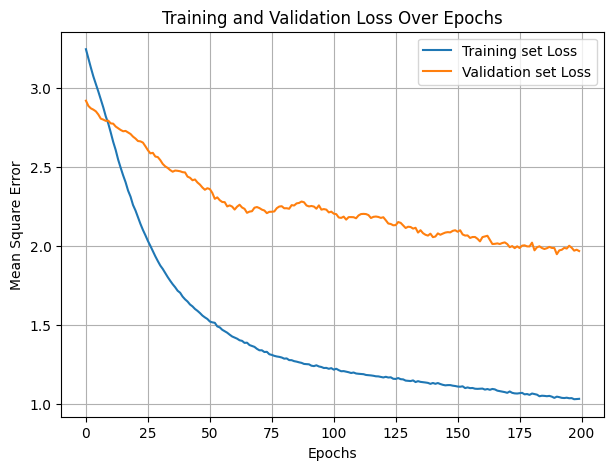
\includegraphics[width=0.4\textwidth]{figures/output1.png}
        \label{fig:subfig1}    
    } \vfill
    \subfigure[Model trained on $80\% \text{ of } 20^3 = 6400$ data points]{
        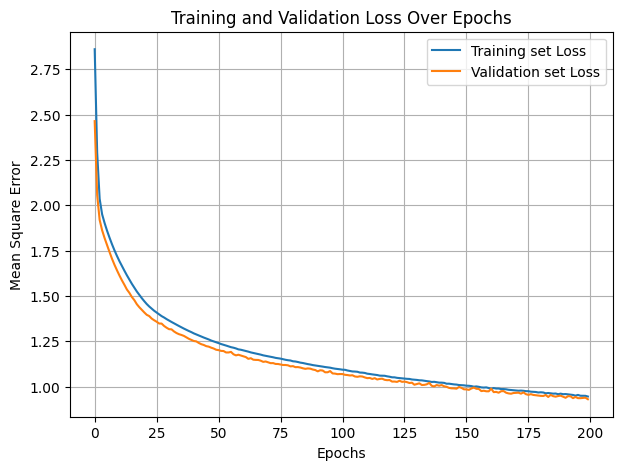
\includegraphics[width=0.4\textwidth]{figures/output5.png}
        \label{fig:subfig2}    
    }
    \caption{Result of the neural network model: Evolution of loss function (MSE) over epochs}
    \label{fig:prob5a}
\end{figure}

% \begin{figure}[htbp]
%     \centerline{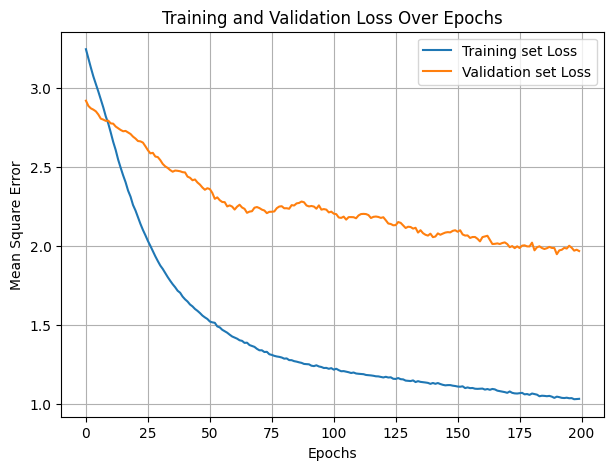
\includegraphics[width=0.4\textwidth]{figures/output1.png}}
%     \caption{Result of the neural network model: Evolution of loss function (MSE) over epochs - Model trained on $80\% \text{ of } 20 = 16$ data points}
%     \label{fig:prob5a}
% \end{figure}

% \begin{figure}[htbp]
%     \centerline{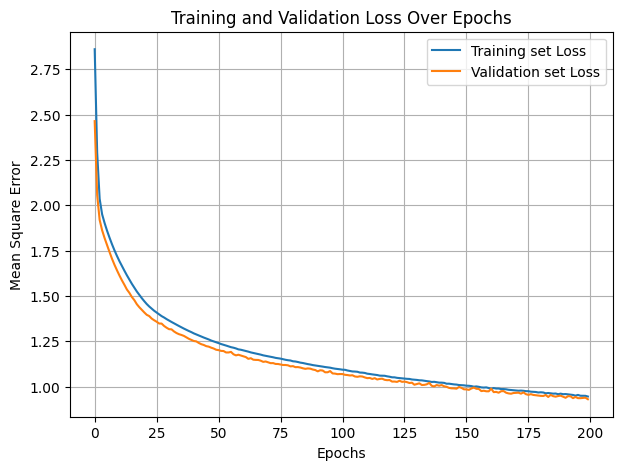
\includegraphics[width=0.4\textwidth]{figures/output5.png}}
%     \caption{Result of the neural network model: Evolution of loss function (MSE) over epochs - Model trained on $80\% \text{ of } 20^3 = 6400$ data points}
%     \label{fig:prob5b}
% \end{figure}

In the end, as a demonstration of the agent's performance, its prediction is compared with the actual values derived from the following IKP equations at time step $t = 0$. Here's the \textit{inverse kinematic problem} equations of the 3-DOF serial robot under review in this problem, obtained in \textit{problem 1} of \textit{homework 4}:

\begin{align}
     & \theta_1 = \frac{\pi}{4} + \frac{\pi}{9} \sin\left(\frac{\pi}{5} t\right)     \\
     & \theta_2 = \frac{\pi}{6} + \frac{\pi}{18} \cos\left(\frac{\pi}{10} t\right)   \\
     & \theta_3 = - \frac{\pi}{9} - \frac{\pi}{36} \sin\left(\frac{\pi}{15} t\right)
\end{align}

And here's the results obtained from the first \_weaker\_ model trained with 16 samples:

\begin{mylistingbox}
    \begin{lstlisting}
    Predicted thetas at t:0 = [0.6419082  0.78249395 0.01114409]
    Actual thetas at t:0 	= [ 0.7854   0.69813 -0.34907]
    Mean Square Error for the test sample at t:0 = 0.052487
    \end{lstlisting}
\end{mylistingbox}

And here's the results obtained from the second \_stronger\_ model trained with 6400 samples:

\begin{mylistingbox}
    \begin{lstlisting}
    Predicted thetas at t:0 = [ 1.2475674   0.1718376  -0.17899337]
    Actual thetas at t:0 	= [ 0.7854   0.69813 -0.34907]
    Mean Square Error for the test sample at t:0 = 0.173169
    \end{lstlisting}
\end{mylistingbox}


% \begin{figure}[htbp]
%     \centerline{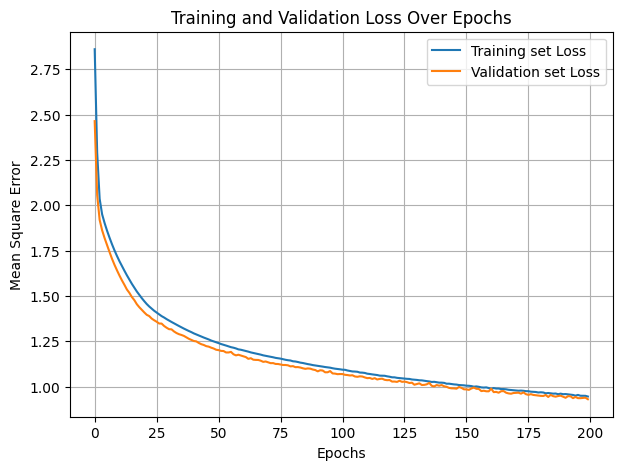
\includegraphics[width=0.4\textwidth]{figures/output5.png}}
%     \caption{Result of the neural network model: Evolution of loss function (MSE) over epochs - Model trained on $80\% \text{ of } 20^3 = 6400$ data points}
%     \label{fig:prob5b}
% \end{figure}



\begin{figure}[htbp]
    \centering
    \subfigure[Comparison of predicted and actual values of $\theta_1$ as the first output of the model]{
        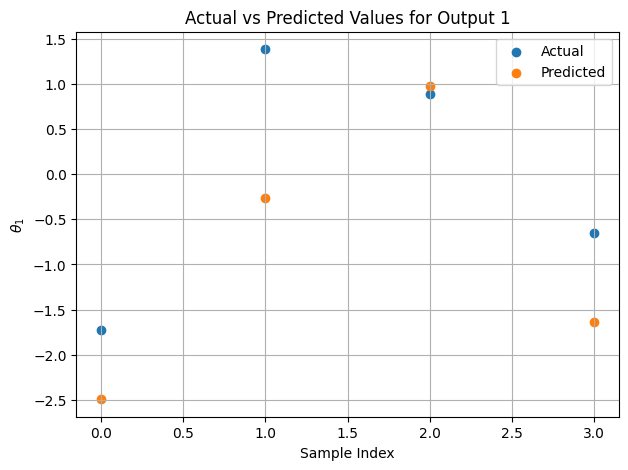
\includegraphics[width=0.4\textwidth]{figures/output2.png}
        % \label{fig:subfig2}    
    } \vfill
    \subfigure[Comparison of predicted and actual values of $\theta_2$ as the second output of the model]{
        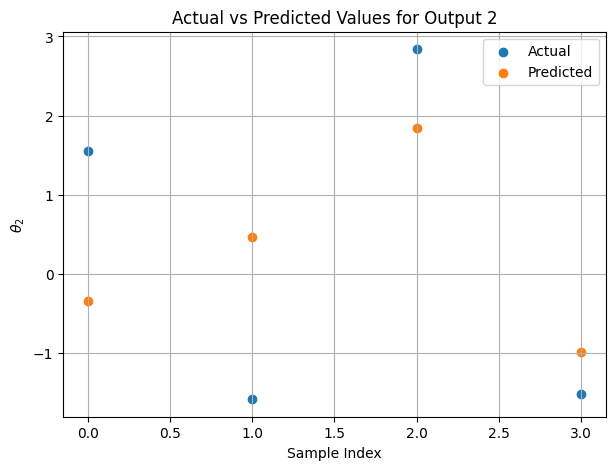
\includegraphics[width=0.4\textwidth]{figures/output3.png}
        % \label{fig:subfig2}    
    } \hfill
    \subfigure[Comparison of predicted and actual values of $\theta_3$ as the third output of the model]{
        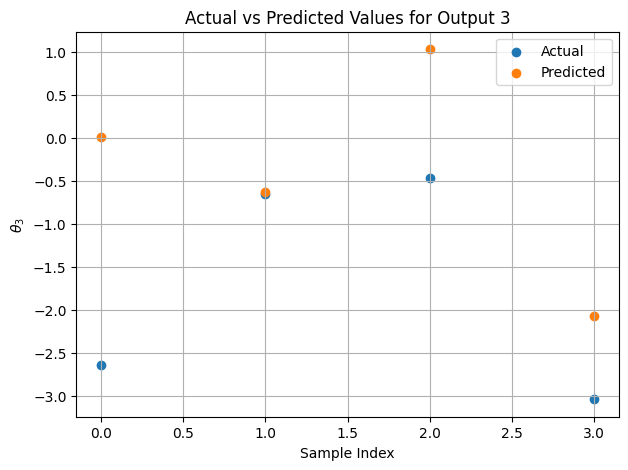
\includegraphics[width=0.4\textwidth]{figures/output4.png}
        % \label{fig:subfig2}    
    }
    \caption{Result of the neural network model: Investigation of the accuracy of predictions}
    \label{fig:prob5b}
\end{figure}

\vspace{20px}

\section{Conclusion}
\textbf{The use of machine learning techniques such as backpropagation, perceptron learning, CNNs, MLPs for IKP, and SVMs in robotics significantly improves data processing and decision-making capabilities. These methods enable robots to perform complex tasks with greater precision and autonomy. Continued development in these areas is essential for future advancements in robotic systems, leading to more intelligent and adaptable robots.}
\vspace{20px}

\begin{thebibliography}{00}
    \bibitem{b1} J. Angeles, ``Fundamentals of Robotic Mechanical Systems'', Theory, Methods, and Algorithms, 4th edition, Springer.

    \bibitem{b2} J. J. Craig, ``Introduction to Robotics'', 3d edition, Pearson Education, Inc.

    \bibitem{b3} A. Chakraborty, Arc - Towards Data Science, ``Derivative of the Sigmoid function'', [Online]. Available: \url{https://towardsdatascience.com/derivative-of-the-sigmoid-function-536880cf918e}

    \bibitem{b4} Wikipedia. 2024. "Rectifier (Neural Networks)." Wikimedia Foundation. Last modified April 30, 2024. \url{https://en.wikipedia.org/wiki/Rectifier_(neural_networks)}.

    \bibitem{b5} B. Krishnamurthy, ``An Introduction to the ReLU Activation Function'', \url{https://builtin.com/machine-learning/relu-activation-function}

    \bibitem{b6} A. Kalhor, ``Neural Networks and Deep Learning'', course pamphlet, School of Electrical and Computer Engineering, University of Tehran, Spring 2023

    \bibitem{b7} H. Hoseini, ``AI in Robotics'', course pamphlet, University of Tehran, Spring 2024

    \bibitem{b8} Simplilearn, ``Support Vector Machine'', \url{https://www.youtube.com/watch?v=TtKF996oEl8}
\end{thebibliography}

\end{document}

% \section{LaTeX Snippets}
% \begin{figure}[htbp]
%     \centerline{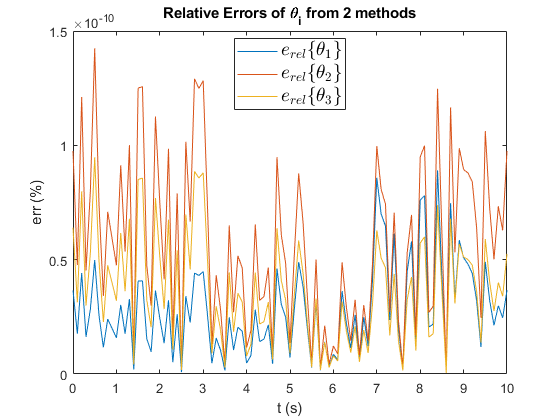
\includegraphics[width=0.4\textwidth]{figures/prob1a.png}}
%     \caption{The differences between joint space angles computed directly and from IKP equations.}
%     \label{fig:res1}
% \end{figure}


% Switch to single-column mode
% \twocolumn[
%     \begin{center}
%             \setstretch{3} % Change the multiplier to control the line height
%             \begin{align}
%                  & {\scriptstyle q_1 = x_1, Q_1 = F_1} \rightarrow
%                  & m_c \ddot{x}_1+m_p\left(\ddot{x}_1+l\left(\dot{\theta}_1^2 \sin \theta_1-\ddot{\theta}_1 \cos \theta_1\right)\right)-k\frac{\left(x_1+x_2\right)\left(\sqrt{\left(x_1+x_2\right)^2+l^2}-l\right)}{\sqrt{\left(x_1+x_2\right)^2+l^2}}=F_1 \\
%                  & {\scriptstyle q_2 = x_2, Q_2 = F_2} \rightarrow
%                  & m_c \ddot{x}_2+m_p\left(\ddot{x}_2+l\left(\dot{\theta}_2^2 \sin \theta_2-\ddot{\theta}_2 \cos \theta_2\right)\right)-k\frac{\left(x_1+x_2\right)\left(\sqrt{\left(x_1+x_2\right)^2+l^2}-l\right)}{\sqrt{\left(x_1+x_2\right)^2+l^2}}=F_2 \\
%                  & {\scriptstyle q_3 = \theta_1, Q_3 = M_1} \rightarrow
%                  & m_p l\left(l \ddot{\theta}_1 - \ddot{x}_1 \cos \left(\theta_1\right) + g \sin \left(\theta_1\right)\right)=M_1                                                                                                                           \\
%                  & {\scriptstyle q_4 = \theta_2, Q_4 = M_1} \rightarrow
%                  & m_p l\left(l \ddot{\theta}_2 - \ddot{x}_2 \cos \left(\theta_2\right) + g \sin \left(\theta_2\right)\right)=M_2
%             \end{align}
%     \end{center}
%     \vspace{22px}
% ]
% \footnotetext{The \textit{gravitational potential energy} of carts is excluded in this equation. That's because the carts move only horizontally and don't have height alternation. Since we are finally going to use the differentiate of the \textit{Lagrangian} with respect to the system's degrees of freedom, these constant terms of ``potential energies of carts'' will be omitted. Therefore, we've ignored them from the very beginning.}

% \begin{table}[htbp]
%     \caption{The D-H parameters of the robot under review}
%     \def\arraystretch{1.45}
%     \begin{center}
%         \begin{tabular}{|Y|Y|Y|Y|Y|}
%             \hline
%             $i$ & $a_i$ & $b_i$ & $\alpha_i$ & $\theta_i$ \\
%             \hline
%             1   & 0     & a     & $\pi / 2$  & $\theta_1$ \\
%             \hline
%             2   & c     & b     & 0          & $\theta_2$ \\
%             \hline
%         \end{tabular}
%     \end{center}
% \end{table}
